% answers.tex —— 2005 年·普通高等学校招生考试·广东卷 · 参考答案与详细解析片段
% 由 tools/generate_projects.py 依来源总账自 2005/2005_数学真题_广东_试题.md + 2005/2005_数学真题_广东_解析正文.md + 2005/2005_数学真题_广东_答案要点.md 生成，勿手改（改源 MD 后重跑）

\begin{answer}
\gksolhead{1}{}

\textbf{题目}：

若集合 $M = \{x \mid |x| \leqslant 2\}$，$N = \{x \mid x^2 - 3x = 0\}$，则 $M \cap N =$\mbox{（　　）}

\begin{gkopts}(4)
\task A．$\{3\}$
\task B．$\{0\}$
\task C．$\{0, 2\}$
\task D．$\{0, 3\}$
\end{gkopts}

\Needspace{4\baselineskip}
\textbf{解析}

由集合 $M = \{x \mid |x| \leqslant 2\} = [-2, 2]$，
解二次方程 $x^2 - 3x = 0 \implies x(x - 3) = 0$，
得集合 $N = \{0, 3\}$．
取两集合的交集：
$0 \in [-2, 2]$，$3 \notin [-2, 2]$，
故 $M \cap N = \{0\}$．
故选 B．

\gkanswer{答案：B}

\end{answer}
\begin{answer}
\gksolhead{2}{}

\textbf{题目}：

若 $(a - 2\mathrm{i})\mathrm{i} = b - \mathrm{i}$，其中 $a, b \in \mathbf{R}$，$\mathrm{i}$ 是虚数单位，则 $a^2 + b^2 =$\mbox{（　　）}

\begin{gkopts}(4)
\task A．$0$
\task B．$2$
\task C．$\dfrac{5}{2}$
\task D．$5$
\end{gkopts}

\Needspace{4\baselineskip}
\textbf{解析}

\Needspace{5\baselineskip}
由题设 $(a - 2\mathrm{i})\mathrm{i} = b - \mathrm{i}$，展开左边：
\nopagebreak[4]
\[
a\mathrm{i} - 2\mathrm{i}^2 = a\mathrm{i} - 2(-1) = 2 + a\mathrm{i}.
\]
\Needspace{5\baselineskip}
因为 $a, b \in \mathbf{R}$，由复数相等的充要条件（实部与虚部分别相等），得：
\nopagebreak[4]
\[
\begin{cases}
b = 2, \\
a = -1.
\end{cases}
\]
\Needspace{5\baselineskip}
所以：
\nopagebreak[4]
\[
a^2 + b^2 = (-1)^2 + 2^2 = 1 + 4 = 5.
\]
故选 D．

\gkanswer{答案：D}

\end{answer}
\begin{answer}
\gksolhead{3}{}

\textbf{题目}：

$\lim\limits_{x\to-3} \dfrac{x + 3}{x^2 - 9} =$\mbox{（　　）}

\begin{gkopts}(4)
\task A．$-\dfrac{1}{6}$
\task B．$0$
\task C．$\dfrac{1}{6}$
\task D．$\dfrac{1}{3}$
\end{gkopts}

\Needspace{4\baselineskip}
\textbf{解析}

\Needspace{5\baselineskip}
将分母进行因式分解：
\nopagebreak[4]
\[
x^2 - 9 = (x + 3)(x - 3).
\]
\Needspace{5\baselineskip}
当 $x \to -3$ 时，$x + 3 \neq 0$，约去公因式：
\nopagebreak[4]
\[
\lim_{x\to-3} \frac{x + 3}{x^2 - 9} = \lim_{x\to-3} \frac{x + 3}{(x + 3)(x - 3)} = \lim_{x\to-3} \frac{1}{x - 3} = \frac{1}{-3 - 3} = -\frac{1}{6}.
\]
故选 A．

\gkanswer{答案：A}

\end{answer}
\begin{answer}
\gksolhead{4}{}

\textbf{题目}：

已知高为 3 的直棱柱 $ABC - A'B'C'$ 的底面是边长为 1 的正三角形（如图所示），则三棱锥 $B' - ABC$ 的体积为\mbox{（　　）}
\nopagebreak[4]
\begin{center}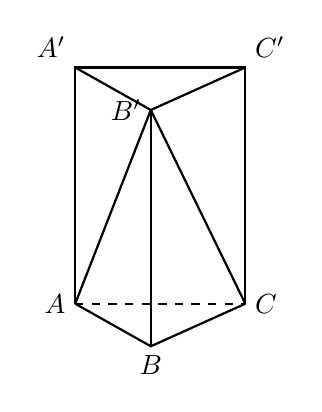
\begin{tikzpicture}[>=stealth, scale=1.2]
  % 顶点定义
  \coordinate (A) at (0, 0);
  \coordinate (B) at (0.8, -0.45);
  \coordinate (C) at (1.8, 0);
  \coordinate (A1) at (0, 2.5);
  \coordinate (B1) at (0.8, 2.05);
  \coordinate (C1) at (1.8, 2.5);

  % 底面和侧棱
  \draw[dashed, thick] (A) -- (C);
  \draw[thick] (A) -- (B) -- (C);
  \draw[thick] (A) -- (A1) -- (C1) -- (C);
  \draw[thick] (B) -- (B1);
  \draw[thick] (A1) -- (B1) -- (C1);

  % 三棱锥 B'-ABC 内部连线
  \draw[thick] (B1) -- (A);
  \draw[thick] (B1) -- (C);

  % 标签
  \node[left] at (A) {$A$};
  \node[below] at (B) {$B$};
  \node[right] at (C) {$C$};
  \node[above left] at (A1) {$A'$};
  \node[left] at (B1) {$B'$};
  \node[above right] at (C1) {$C'$};
\end{tikzpicture}
\end{center}
\nopagebreak[4]
\begin{gkopts}(2)
\task A．$\dfrac{1}{4}$
\task B．$\dfrac{1}{2}$
\task C．$\dfrac{\sqrt{3}}{6}$
\task D．$\dfrac{\sqrt{3}}{4}$
\end{gkopts}

\Needspace{4\baselineskip}
\textbf{解析}

直棱柱 $ABC - A'B'C'$ 的高为 $h = 3$．
\Needspace{5\baselineskip}
底面 $\triangle ABC$ 为边长为 $1$ 的正三角形，其面积为：
\nopagebreak[4]
\[
S_{\triangle ABC} = \frac{\sqrt{3}}{4} \times 1^2 = \frac{\sqrt{3}}{4}.
\]
因为 $B'B$ 垂直于底面 $ABC$，所以点 $B'$ 到底面 $ABC$ 的距离等于直棱柱的高 $h = 3$．
\Needspace{5\baselineskip}
三棱锥 $B' - ABC$ 的体积为：
\nopagebreak[4]
\[
V = \frac{1}{3} S_{\triangle ABC} \cdot h = \frac{1}{3} \times \frac{\sqrt{3}}{4} \times 3 = \frac{\sqrt{3}}{4}.
\]
故选 D．

\gkanswer{答案：D}

\end{answer}
\begin{answer}
\gksolhead{5}{}

\textbf{题目}：

若焦点在 $x$ 轴上的椭圆 $\dfrac{x^2}{2} + \dfrac{y^2}{m} = 1$ 的离心率为 $\dfrac{1}{2}$，则 $m =$\mbox{（　　）}

\begin{gkopts}(4)
\task A．$\sqrt{3}$
\task B．$\dfrac{3}{2}$
\task C．$\dfrac{8}{3}$
\task D．$\dfrac{2}{3}$
\end{gkopts}

\Needspace{4\baselineskip}
\textbf{解析}

已知椭圆方程为 $\dfrac{x^2}{2} + \dfrac{y^2}{m} = 1$．
因为焦点在 $x$ 轴上，所以 $a^2 = 2$，$b^2 = m$，且 $0 < m < 2$．
\Needspace{5\baselineskip}
半焦距为 $c$，由离心率 $e = \dfrac{c}{a} = \dfrac{1}{2}$，得：
\nopagebreak[4]
\[
c^2 = \frac{1}{4} a^2 = \frac{1}{4} \times 2 = \frac{1}{2}.
\]
\Needspace{5\baselineskip}
由椭圆几何性质 $b^2 = a^2 - c^2$，得：
\nopagebreak[4]
\[
m = 2 - \frac{1}{2} = \frac{3}{2}.
\]
故选 B．

\gkanswer{答案：B}

\end{answer}
\begin{answer}
\gksolhead{6}{}

\textbf{题目}：

函数 $f(x) = x^3 - 3x^2 + 1$ 是减函数的区间为\mbox{（　　）}

\begin{gkopts}(4)
\task A．$(2, +\infty)$
\task B．$(-\infty, 2)$
\task C．$(-\infty, 0)$
\task D．$(0, 2)$
\end{gkopts}

\Needspace{4\baselineskip}
\textbf{解析}

\Needspace{5\baselineskip}
函数 $f(x) = x^3 - 3x^2 + 1$ 的导数为：
\nopagebreak[4]
\[
f'(x) = 3x^2 - 6x = 3x(x - 2).
\]
\Needspace{5\baselineskip}
令 $f'(x) < 0$，即：
\nopagebreak[4]
\[
3x(x - 2) < 0 \iff 0 < x < 2.
\]
所以函数 $f(x)$ 的单调递减区间为 $(0, 2)$．
故选 D．

\gkanswer{答案：D}

\end{answer}
\begin{answer}
\gksolhead{7}{}

\textbf{题目}：

给出下列关于互不相同的直线 $m$、$l$、$n$ 和平面 $\alpha$、$\beta$ 的四个命题：

① 若 $m \subset \alpha, l \cap \alpha = A, A \notin m$，则 $l$ 与 $m$ 不共面；

② 若 $m$、$l$ 是异面直线，$l \parallel \alpha, m \parallel \alpha$，且 $n \perp l, n \perp m$，则 $n \perp \alpha$；

③ 若 $l \parallel \alpha, m \parallel \beta, \alpha \parallel \beta$，则 $l \parallel m$；

④ 若 $l \subset \alpha, m \subset \alpha, l \cap m = A, l \parallel \beta, m \parallel \beta$，则 $\alpha \parallel \beta$．

其中为假命题的是\mbox{（　　）}

\begin{gkopts}(4)
\task A．①
\task B．②
\task C．③
\task D．④
\end{gkopts}

\Needspace{4\baselineskip}
\textbf{解析}

逐项辨析各命题：
\begin{itemize}
\item 命题 ①：若 $m \subset \alpha, l \cap \alpha = A, A \notin m$，根据异面直线的判定定理，经过平面外一点和平面内一点的直线，与平面内不经过该点的直线互为异面直线，故 $l$ 与 $m$ 不共面，为真命题；
\item 命题 ②：若 $m, l$ 是异面直线，$l \parallel \alpha, m \parallel \alpha$，则异面直线 $l, m$ 的方向向量所确定的平面平行于 $\alpha$．因为 $n \perp l$ 且 $n \perp m$，所以直线 $n$ 垂直于由 $l, m$ 方向向量平移构成的相交直线所确定的平面，故必有 $n \perp \alpha$，为真命题；
\item 命题 ③：若 $l \parallel \alpha, m \parallel \beta, \alpha \parallel \beta$，则直线 $l$ 与 $m$ 平行于同一组平行平面，空间中 $l$ 与 $m$ 的位置关系可以平行、相交或异面，并不必然平行，故为假命题；
\item 命题 ④：若 $l \subset \alpha, m \subset \alpha, l \cap m = A, l \parallel \beta, m \parallel \beta$，根据两平面平行的判定定理，一个平面内有两条相交直线都平行于另一个平面，则两平面互相平行，故为真命题．
\end{itemize}

综上所述，假命题为 ③．
故选 C．

\gkanswer{答案：C}

\end{answer}
\begin{answer}
\gksolhead{8}{}

\textbf{题目}：

先后抛掷两枚均匀的正方体骰子（它们的六个面分别标有点数 1、2、3、4、5、6），骰子朝上的面的点数分别为 $X$、$Y$，则 $\log_{2X} Y = 1$ 的概率为\mbox{（　　）}

\begin{gkopts}(4)
\task A．$\dfrac{1}{6}$
\task B．$\dfrac{5}{36}$
\task C．$\dfrac{1}{12}$
\task D．$\dfrac{1}{2}$
\end{gkopts}

\Needspace{4\baselineskip}
\textbf{解析}

\Needspace{5\baselineskip}
先后抛掷两枚骰子，试验的样本空间包含的样本点总数为：
\nopagebreak[4]
\[
n = 6 \times 6 = 36.
\]
\Needspace{5\baselineskip}
由对数方程 $\log_{2X} Y = 1$，得：
\nopagebreak[4]
\[
Y = 2X.
\]
由于 $X, Y \in \{1, 2, 3, 4, 5, 6\}$，满足条件的点对 $(X, Y)$ 共有：
\begin{itemize}
\item 当 $X = 1$ 时，$Y = 2$；
\item 当 $X = 2$ 时，$Y = 4$；
\item 当 $X = 3$ 时，$Y = 6$．
\end{itemize}

共有 3 种结果．
\Needspace{5\baselineskip}
所以所求概率为：
\nopagebreak[4]
\[
P = \frac{3}{36} = \frac{1}{12}.
\]
故选 C．

\gkanswer{答案：C}

\end{answer}
\begin{answer}
\gksolhead{9}{}

\textbf{题目}：

在同一平面直角坐标系中，函数 $y = f(x)$ 和 $y = g(x)$ 的图象关于直线 $y = x$ 对称．现将 $y = g(x)$ 的图象沿 $x$ 轴向左平移 2 个单位，再沿 $y$ 轴向上平移 1 个单位，所得的图象是由两条线段组成的折线（如图所示），则函数 $f(x)$ 的表达式为\mbox{（　　）}
\nopagebreak[4]
\begin{center}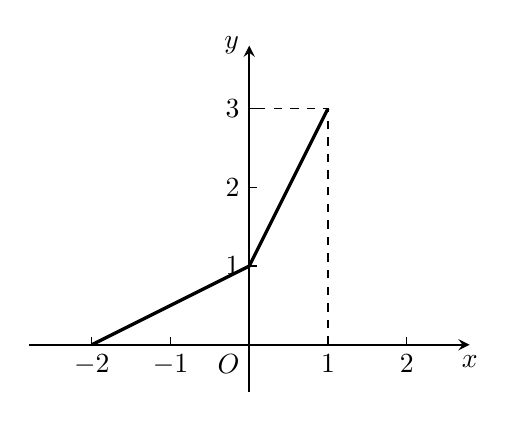
\begin{tikzpicture}[>=stealth, scale=1.0]
  % 坐标轴
  \draw[->, thick] (-2.8, 0) -- (2.8, 0) node[below] {$x$};
  \draw[->, thick] (0, -0.6) -- (0, 3.8) node[left] {$y$};
  \node[below left] at (0, 0) {$O$};

  % 刻度
  \foreach \x in {-2, -1, 1, 2} {
    \draw (\x, 0) -- (\x, 0.1);
    \node[below] at (\x, 0) {$\x$};
  }
  \foreach \y in {1, 2, 3} {
    \draw (0, \y) -- (0.1, \y);
    \node[left] at (0, \y) {$\y$};
  }

  % 虚线辅助线
  \draw[dashed] (1, 0) -- (1, 3) -- (0, 3);

  % 折线
  \draw[very thick] (-2, 0) -- (0, 1) -- (1, 3);
\end{tikzpicture}
\end{center}
\nopagebreak[4]
\begin{gkopts}(1)
\task A．$f(x) = \begin{cases} 2x + 2, & -1 \leqslant x \leqslant 0, \\ \dfrac{x}{2} + 2, & 0 < x \leqslant 2 \end{cases}$
\task B．$f(x) = \begin{cases} 2x - 2, & -1 \leqslant x \leqslant 0, \\ \dfrac{x}{2} - 2, & 0 < x \leqslant 2 \end{cases}$
\task C．$f(x) = \begin{cases} 2x - 2, & 1 \leqslant x \leqslant 2, \\ \dfrac{x}{2} + 1, & 2 < x \leqslant 4 \end{cases}$
\task D．$f(x) = \begin{cases} 2x - 6, & 1 \leqslant x \leqslant 2, \\ \dfrac{x}{2} - 3, & 2 < x \leqslant 4 \end{cases}$
\end{gkopts}

\Needspace{4\baselineskip}
\textbf{解析}

设平移后得到的函数为 $h(x)$．
\Needspace{5\baselineskip}
根据题意，$h(x)$ 的图象是由 $y = g(x)$ 的图象沿 $x$ 轴向左平移 2 个单位、再沿 $y$ 轴向上平移 1 个单位得到的，因此：
\nopagebreak[4]
\[
h(x) = g(x + 2) + 1 \implies g(x) = h(x - 2) - 1.
\]
因为函数 $y = f(x)$ 与 $y = g(x)$ 的图象关于直线 $y = x$ 对称，所以 $f(x)$ 与 $g(x)$ 互为反函数．
根据题图，折线 $h(x)$ 上的三个特征关键点为：
起点 $A_h(-2, 0)$、拐点 $B_h(0, 1)$、终点 $C_h(1, 3)$．
\Needspace{5\baselineskip}
追踪各点在 $g(x)$ 上的对应坐标（横坐标加 2，纵坐标减 1）：
\nopagebreak[4]
\[
\begin{aligned}
A_g(0, -1) &\in g, \\
B_g(2, 0) &\in g, \\
C_g(3, 2) &\in g.
\end{aligned}
\]
\Needspace{5\baselineskip}
由于 $f$ 与 $g$ 互为反函数，将各点横纵坐标互换，得到 $f(x)$ 图象上的对应点：
\nopagebreak[4]
\[
\begin{aligned}
A_f(-1, 0) &\in f, \\
B_f(0, 2) &\in f, \\
C_f(2, 3) &\in f.
\end{aligned}
\]
因此函数 $f(x)$ 的定义域为 $[-1, 2]$：
\begin{itemize}
\item 当 $-1 \leqslant x \leqslant 0$ 时，过点 $(-1, 0)$ 与 $(0, 2)$，斜率为 $\dfrac{2 - 0}{0 - (-1)} = 2$，直线方程为 $y = 2x + 2$；
\item 当 $0 < x \leqslant 2$ 时，过点 $(0, 2)$ 与 $(2, 3)$，斜率为 $\dfrac{3 - 2}{2 - 0} = \dfrac{1}{2}$，直线方程为 $y = \dfrac{x}{2} + 2$．
\end{itemize}

\Needspace{5\baselineskip}
写成分段函数形式：
\nopagebreak[4]
\[
f(x) = \begin{cases}
2x + 2, & -1 \leqslant x \leqslant 0, \\
\dfrac{x}{2} + 2, & 0 < x \leqslant 2.
\end{cases}
\]
故选 A．

\gkanswer{答案：A}

\end{answer}
\begin{answer}
\gksolhead{10}{}

\textbf{题目}：

已知数列 $\{x_n\}$ 满足 $x_2 = \dfrac{x_1}{2}$，$x_n = \dfrac{1}{2}(x_{n-1} + x_{n-2}), n = 3, 4, \dots$．若 $\lim\limits_{n\to\infty} x_n = 2$，则 $x_1 =$\mbox{（　　）}

\begin{gkopts}(4)
\task A．$\dfrac{3}{2}$
\task B．$3$
\task C．$4$
\task D．$5$
\end{gkopts}

\Needspace{4\baselineskip}
\textbf{解析}

\Needspace{5\baselineskip}
数列递推关系为：
\nopagebreak[4]
\[
x_n = \frac{1}{2}(x_{n-1} + x_{n-2}) \quad (n \geqslant 3).
\]
\Needspace{5\baselineskip}
两边同减去 $x_{n-1}$，得：
\nopagebreak[4]
\[
x_n - x_{n-1} = -\frac{1}{2}(x_{n-1} - x_{n-2}).
\]
因此差分数列 $\{x_{k+1} - x_k\}$ 是以首项 $x_2 - x_1$、公比为 $-\dfrac{1}{2}$ 的等比数列．
\Needspace{5\baselineskip}
由 $x_2 = \dfrac{x_1}{2}$，得首项为：
\nopagebreak[4]
\[
x_2 - x_1 = \frac{x_1}{2} - x_1 = -\frac{x_1}{2}.
\]
\Needspace{5\baselineskip}
对差分式进行累加：
\nopagebreak[4]
\[
x_n = x_1 + \sum_{k=1}^{n-1} (x_{k+1} - x_k) = x_1 + (x_2 - x_1) \sum_{j=0}^{n-2} \left(-\frac{1}{2}\right)^j.
\]
\Needspace{5\baselineskip}
当 $n \to \infty$ 时，等比级数求和收敛：
\nopagebreak[4]
\[
\lim_{n\to\infty} x_n = x_1 + \frac{x_2 - x_1}{1 - \left(-\frac{1}{2}\right)} = x_1 + \frac{-\frac{x_1}{2}}{\frac{3}{2}} = x_1 - \frac{1}{3}x_1 = \frac{2}{3}x_1.
\]
\Needspace{5\baselineskip}
已知 $\lim\limits_{n\to\infty} x_n = 2$，即：
\nopagebreak[4]
\[
\frac{2}{3}x_1 = 2 \implies x_1 = 3.
\]
故选 B．

\gkanswer{答案：B}

\end{answer}
\begin{answer}
\gksolhead{11}{}

\textbf{题目}：

函数 $f(x) = \dfrac{1}{\sqrt{1 - \mathrm{e}^x}}$ 的定义域是 $\underline{\qquad}$．

\Needspace{4\baselineskip}
\textbf{解析}

\Needspace{5\baselineskip}
要使函数 $f(x) = \dfrac{1}{\sqrt{1 - \mathrm{e}^x}}$ 有意义，根号下式子必须严格大于 0：
\nopagebreak[4]
\[
1 - \mathrm{e}^x > 0 \iff \mathrm{e}^x < 1 \iff x < 0.
\]
所以函数的定义域为 $(-\infty, 0)$．

\gkanswer{答案：$(-\infty, 0)$}

\end{answer}
\begin{answer}
\gksolhead{12}{}

\textbf{题目}：

已知向量 $\vec{a} = (2, 3), \vec{b} = (x, 6)$，且 $\vec{a} \parallel \vec{b}$，则 $x = \underline{\qquad}$．

\Needspace{4\baselineskip}
\textbf{解析}

已知向量 $\vec{a} = (2, 3), \vec{b} = (x, 6)$．
\Needspace{5\baselineskip}
因为 $\vec{a} \parallel \vec{b}$，所以坐标交叉相乘之差为 0：
\nopagebreak[4]
\[
2 \times 6 - 3 \times x = 0 \iff 12 - 3x = 0 \iff x = 4.
\]

\gkanswer{答案：$4$}

\end{answer}
\begin{answer}
\gksolhead{13}{}

\textbf{题目}：

已知 $(x\cos\theta + 1)^5$ 的展开式中 $x^2$ 的系数与 $\left(x + \dfrac{5}{4}\right)^4$ 的展开式中 $x^3$ 的系数相等，则 $\cos\theta = \underline{\qquad}$．

\Needspace{4\baselineskip}
\textbf{解析}

\Needspace{5\baselineskip}
$(x\cos\theta + 1)^5$ 的二项展开式通项为：
\nopagebreak[4]
\[
T_{r+1} = \mathrm{C}_5^r (x\cos\theta)^{5-r} \cdot 1^r.
\]
\Needspace{5\baselineskip}
令 $5 - r = 2 \implies r = 3$，得到 $x^2$ 的项：
\nopagebreak[4]
\[
T_4 = \mathrm{C}_5^3 (x\cos\theta)^2 \cdot 1^3 = 10 \cos^2\theta \cdot x^2.
\]
其系数为 $10\cos^2\theta$．
\Needspace{5\baselineskip}
$\left(x + \dfrac{5}{4}\right)^4$ 的二项展开式通项为：
\nopagebreak[4]
\[
T'_{k+1} = \mathrm{C}_4^k x^{4-k} \left(\frac{5}{4}\right)^k.
\]
\Needspace{5\baselineskip}
令 $4 - k = 3 \implies k = 1$，得到 $x^3$ 的项：
\nopagebreak[4]
\[
T'_2 = \mathrm{C}_4^1 x^3 \cdot \left(\frac{5}{4}\right)^1 = 4 \times \frac{5}{4} x^3 = 5 x^3.
\]
其系数为 $5$．
\Needspace{5\baselineskip}
由题意，两系数相等：
\nopagebreak[4]
\[
10\cos^2\theta = 5 \implies \cos^2\theta = \frac{1}{2} \implies \cos\theta = \pm \frac{\sqrt{2}}{2}.
\]

\gkanswer{答案：$\pm \dfrac{\sqrt{2}}{2}$}

\end{answer}
\begin{answer}
\gksolhead{14}{}

\textbf{题目}：

设平面内有 $n$ 条直线 ($n \geqslant 3$)，其中有且仅有两条直线互相平行，任意三条直线不过同一点．若用 $f(n)$ 表示这 $n$ 条直线交点的个数，则 $f(4) = \underline{\qquad}$；当 $n > 4$ 时，$f(n) = \underline{\qquad}$．（用 $n$ 表示）

\Needspace{4\baselineskip}
\textbf{解析}

若平面内 $n$ 条直线两两相交且任意三条不过同一点，则交点总数为 $\mathrm{C}_n^2 = \dfrac{n(n-1)}{2}$．
题设 $n$ 条直线中有且仅有两条直线互相平行，其余任意两条直线均相交，且任意三条直线不过同一点．
\Needspace{5\baselineskip}
因此交点个数恰比完全两两相交的情形减少 1 个：
\nopagebreak[4]
\[
f(n) = \mathrm{C}_n^2 - 1 = \frac{n(n-1)}{2} - 1.
\]
\Needspace{5\baselineskip}
当 $n = 4$ 时：
\nopagebreak[4]
\[
f(4) = \frac{4 \times 3}{2} - 1 = 6 - 1 = 5.
\]
当 $n > 4$ 时，交点个数为 $\dfrac{n(n-1)}{2} - 1$．

\gkanswer{答案：$5$；$\dfrac{n(n-1)}{2} - 1$}

\end{answer}
\begin{answer}
\gksolhead{15}{}

\textbf{题目}：

化简 $f(x) = \cos\left(\dfrac{6k+1}{3}\pi + 2x\right) + \cos\left(\dfrac{6k-1}{3}\pi - 2x\right) + 2\sqrt{3}\sin\left(\dfrac{\pi}{3} + 2x\right)$ ($x \in \mathbf{R}, k \in \mathbf{Z}$)，并求函数 $f(x)$ 的值域和最小正周期．

\Needspace{4\baselineskip}
\textbf{解析}

利用诱导公式化简前两项：
\Needspace{5\baselineskip}
因为 $k \in \mathbf{Z}$，
\nopagebreak[4]
\[
\frac{6k+1}{3}\pi + 2x = 2k\pi + \frac{\pi}{3} + 2x,
\]
\Needspace{5\baselineskip}
所以：
\nopagebreak[4]
\[
\cos\left(\frac{6k+1}{3}\pi + 2x\right) = \cos\left(2k\pi + 2x + \frac{\pi}{3}\right) = \cos\left(2x + \frac{\pi}{3}\right).
\]
\Needspace{5\baselineskip}
同理：
\nopagebreak[4]
\[
\frac{6k-1}{3}\pi - 2x = 2k\pi - \left(2x + \frac{\pi}{3}\right),
\]
\Needspace{5\baselineskip}
由余弦函数的偶函数性质：
\nopagebreak[4]
\[
\cos\left(\frac{6k-1}{3}\pi - 2x\right) = \cos\left(2k\pi - \left(2x + \frac{\pi}{3}\right)\right) = \cos\left(-\left(2x + \frac{\pi}{3}\right)\right) = \cos\left(2x + \frac{\pi}{3}\right).
\]
\Needspace{5\baselineskip}
将前两项相加，得：
\nopagebreak[4]
\[
\cos\left(\frac{6k+1}{3}\pi + 2x\right) + \cos\left(\frac{6k-1}{3}\pi - 2x\right) = 2\cos\left(2x + \frac{\pi}{3}\right).
\]
\Needspace{5\baselineskip}
代入原式：
\nopagebreak[4]
\[
f(x) = 2\cos\left(2x + \frac{\pi}{3}\right) + 2\sqrt{3}\sin\left(2x + \frac{\pi}{3}\right).
\]
\Needspace{5\baselineskip}
提取公因数 4：
\nopagebreak[4]
\[
f(x) = 4\left[\frac{1}{2}\cos\left(2x + \frac{\pi}{3}\right) + \frac{\sqrt{3}}{2}\sin\left(2x + \frac{\pi}{3}\right)\right].
\]
\Needspace{5\baselineskip}
引入辅助角公式：
\nopagebreak[4]
\[
f(x) = 4\sin\left(2x + \frac{\pi}{3} + \frac{\pi}{6}\right) = 4\sin\left(2x + \frac{\pi}{2}\right) = 4\cos 2x.
\]
\Needspace{5\baselineskip}
因此化简结果为：
\nopagebreak[4]
\[
f(x) = 4\cos 2x.
\]
由余弦函数的性质：
因为 $\cos 2x \in [-1, 1]$，所以函数 $f(x)$ 的值域为 $[-4, 4]$；
\Needspace{5\baselineskip}
最小正周期为：
\nopagebreak[4]
\[
T = \frac{2\pi}{2} = \pi.
\]

\gkanswer{答案：化简结果为 $f(x) = 4\cos 2x$；值域为 $[-4, 4]$，最小正周期为 $\pi$。}

\end{answer}
\begin{answer}
\gksolhead{16}{}

\textbf{题目}：

如图所示，在四面体 $P - ABC$ 中，已知 $PA = BC = 6, PC = AB = 10, AC = 8, PB = 2\sqrt{34}$．$F$ 是线段 $PB$ 上一点，$CF = \dfrac{15}{17}\sqrt{34}$，点 $E$ 在线段 $AB$ 上，且 $EF \perp PB$．
\nopagebreak[4]
\begin{center}\begin{tikzpicture}[>=stealth, scale=1.1]
  % 顶点坐标
  \coordinate (P) at (0, 3.2);
  \coordinate (A) at (0, 0);
  \coordinate (C) at (2.6, 0);
  \coordinate (B) at (3.4, 1.8);
  \coordinate (F) at ($(P)!0.45!(B)$);
  \coordinate (E) at ($(A)!0.6!(B)$);

  % 轮廓实线
  \draw[thick] (P) -- (A) -- (C) -- (B) -- (P);
  \draw[thick] (P) -- (C);
  \draw[thick] (C) -- (F);

  % 内部虚线
  \draw[dashed, thick] (A) -- (B);
  \draw[dashed, thick] (E) -- (F);
  \draw[dashed, thick] (C) -- (E);

  % 顶点标签
  \node[above] at (P) {$P$};
  \node[below left] at (A) {$A$};
  \node[below right] at (C) {$C$};
  \node[right] at (B) {$B$};
  \node[above right] at (F) {$F$};
  \node[left] at (E) {$E$};
\end{tikzpicture}
\end{center}
\nopagebreak[4]
(1) 证明：$PB \perp \text{\text{平面} } CEF$；

(2) 求二面角 $B - CE - F$ 的大小．

\Needspace{4\baselineskip}
\textbf{解析}

\gksubpart{(1)}

在 $\triangle PAC$ 中，各边长为 $PA = 6, AC = 8, PC = 10$．
因为 $6^2 + 8^2 = 36 + 64 = 100 = 10^2$，
即 $PA^2 + AC^2 = PC^2$，
所以 $\triangle PAC$ 为以 $\angle PAC$ 为直角的直角三角形，即 $PA \perp AC$．

在 $\triangle ABC$ 中，各边长为 $BC = 6, AC = 8, AB = 10$．
因为 $6^2 + 8^2 = 100 = 10^2$，
即 $BC^2 + AC^2 = AB^2$，
所以 $\triangle ABC$ 为以 $\angle ACB$ 为直角的直角三角形，即 $BC \perp AC$．

在 $\triangle PBC$ 中，各边长为 $BC = 6, PC = 10, PB = 2\sqrt{34}$．
因为 $BC^2 + PC^2 = 6^2 + 10^2 = 36 + 100 = 136$，
而 $PB^2 = (2\sqrt{34})^2 = 4 \times 34 = 136$，
即 $BC^2 + PC^2 = PB^2$，
所以 $\triangle PBC$ 为以 $\angle PCB$ 为直角的直角三角形，即 $BC \perp PC$．

\Needspace{5\baselineskip}
在 Rt$\triangle PBC$ 中，斜边 $PB = 2\sqrt{34}$ 上的高为：
\nopagebreak[4]
\[
h = \frac{BC \cdot PC}{PB} = \frac{6 \times 10}{2\sqrt{34}} = \frac{30}{\sqrt{34}} = \frac{15}{17}\sqrt{34}.
\]
已知 $CF = \dfrac{15}{17}\sqrt{34}$，且点 $F$ 在线段 $PB$ 上，
因此 $CF$ 即为斜边 $PB$ 上的高，从而有 $CF \perp PB$．
又已知 $EF \perp PB$，且 $CF \cap EF = F$，$CF, EF \subset \text{\text{平面} } CEF$，
所以 $PB \perp \text{\text{平面} } CEF$．

\gksubpart{(2)}

因为 $AC \perp BC$ 且 $PC \perp BC$，$AC \cap PC = C$，
所以 $BC \perp \text{\text{平面} } PAC$．
又 $AC \subset \text{\text{平面} } PAC$，故 $BC \perp AC$．
以 $C$ 为原点，以射线 $CA, CB$ 方向分别为 $x$ 轴、$y$ 轴正半轴，垂直于底面 $ABC$ 向上的方向为 $z$ 轴正半轴，建立空间直角坐标系 $C - xyz$．

各点坐标为：
$C(0, 0, 0)$，$A(8, 0, 0)$，$B(0, 6, 0)$．
设点 $P$ 的坐标为 $(x_P, y_P, z_P)$．
因为 $BC \perp \text{\text{平面} } PAC$，所以平面 $PAC$ 即为 $xOz$ 坐标平面，故 $y_P = 0$．
又 $PA \perp AC$，且 $CA$ 位于 $x$ 轴上，$C(0,0,0), A(8,0,0)$，
故点 $P$ 在 $x$ 轴上的投影为 $A(8, 0, 0)$，即 $x_P = 8$．
由 $PA = 6$，且点 $P$ 位于底面上方，得 $z_P = 6$．
所以点 $P$ 的坐标为 $(8, 0, 6)$．

向量 $\vec{BP} = (8, -6, 6)$．
由（1）知 $PB \perp \text{\text{平面} } CEF$，故向量 $\vec{BP} = (8, -6, 6)$ 即为平面 $CEF$ 的一个法向量，记为 $\vec{n}_2 = (8, -6, 6)$．
平面 $B - CE$ 即为底面 $ABC$（$xOy$ 坐标平面），其法向量可取为 $\vec{n}_1 = (0, 0, 1)$．

\Needspace{5\baselineskip}
设二面角 $B - CE - F$ 的平面角为 $\theta$（$\theta$ 为锐角），则：
\nopagebreak[4]
\[
\cos\theta = \frac{|\vec{n}_1 \cdot \vec{n}_2|}{|\vec{n}_1| |\vec{n}_2|} = \frac{|6|}{1 \times \sqrt{8^2 + (-6)^2 + 6^2}} = \frac{6}{2\sqrt{34}} = \frac{3\sqrt{34}}{34}.
\]
所以二面角 $B - CE - F$ 的大小为 $\arccos\dfrac{3\sqrt{34}}{34}$．

\gkanswer{答案（1）：证明见解析。}

\gkanswer{答案（2）：$\arccos\dfrac{3\sqrt{34}}{34}$。}

\end{answer}
\begin{answer}
\gksolhead{17}{}

\textbf{题目}：

在平面直角坐标系 $xOy$ 中，抛物线 $y = x^2$ 上异于坐标原点 $O$ 的两不同动点 $A$、$B$ 满足 $AO \perp BO$（如图所示）．
\nopagebreak[4]
\begin{center}\begin{tikzpicture}[>=stealth, scale=1.1]
  % 坐标轴
  \draw[->, thick] (-2.2, 0) -- (2.2, 0) node[below] {$x$};
  \draw[->, thick] (0, -0.6) -- (0, 3.2) node[left] {$y$};
  \node[below left] at (0, 0) {$O$};

  % 抛物线 y = x^2
  \draw[very thick, domain=-1.6:1.6, samples=100] plot (\x, {\x*\x});

  % 点 A 和点 B，满足 x1*x2 = -1
  % 取 x1 = -1.25 -> y1 = 1.5625; x2 = 0.8 -> y2 = 0.64
  \coordinate (O) at (0, 0);
  \coordinate (A) at (-1.25, 1.5625);
  \coordinate (B) at (0.8, 0.64);

  % 弦与连线
  \draw[thick] (O) -- (A) -- (B) -- (O);

  % 直角标志
  \coordinate (P1) at ($(O)!0.15!(A)$);
  \coordinate (P2) at ($(O)!0.15!(B)$);
  \coordinate (P3) at ($(P1) + (P2)$);
  \draw[thin] (P1) -- (P3) -- (P2);

  % 标签
  \node[left] at (A) {$A$};
  \node[right] at (B) {$B$};
\end{tikzpicture}
\end{center}
\nopagebreak[4]
(1) 求 $\triangle AOB$ 的重心 $G$（即三角形三条中线的交点）的轨迹方程；

(2) $\triangle AOB$ 的面积是否存在最小值？若存在，请求出最小值；若不存在，请说明理由．

\Needspace{4\baselineskip}
\textbf{解析}

\gksubpart{(1)}

设抛物线 $y = x^2$ 上的动点坐标为 $A(x_1, y_1)$ 与 $B(x_2, y_2)$，其中 $y_1 = x_1^2, y_2 = x_2^2$．
因为点 $A, B$ 异于坐标原点 $O$，所以 $x_1 \neq 0, x_2 \neq 0$．
\Needspace{5\baselineskip}
由 $AO \perp BO$，得向量数量积：
\nopagebreak[4]
\[
\vec{OA} \cdot \vec{OB} = x_1 x_2 + y_1 y_2 = x_1 x_2 + x_1^2 x_2^2 = x_1 x_2(1 + x_1 x_2) = 0.
\]
\Needspace{5\baselineskip}
因为 $x_1 x_2 \neq 0$，所以：
\nopagebreak[4]
\[
1 + x_1 x_2 = 0 \implies x_1 x_2 = -1.
\]
\Needspace{5\baselineskip}
设 $\triangle AOB$ 的重心为 $G(x, y)$，根据三角形重心坐标公式：
\nopagebreak[4]
\[
\begin{cases}
x = \dfrac{x_1 + x_2 + 0}{3} = \dfrac{x_1 + x_2}{3}, \\
y = \dfrac{y_1 + y_2 + 0}{3} = \dfrac{x_1^2 + x_2^2}{3}.
\end{cases}
\]
由第一式得 $x_1 + x_2 = 3x$．
\Needspace{5\baselineskip}
将第二式中的分子用 $x_1 + x_2$ 与 $x_1 x_2$ 表示：
\nopagebreak[4]
\[
x_1^2 + x_2^2 = (x_1 + x_2)^2 - 2x_1 x_2 = (3x)^2 - 2(-1) = 9x^2 + 2.
\]
\Needspace{5\baselineskip}
代入 $y$ 的表达式：
\nopagebreak[4]
\[
y = \frac{9x^2 + 2}{3} = 3x^2 + \frac{2}{3}.
\]
因为方程 $t^2 - (3x)t - 1 = 0$ 的判别式 $\Delta = 9x^2 + 4 > 0$ 恒成立，所以对于任意 $x \in \mathbf{R}$，都存在相异的两实根 $x_1, x_2$ 使得 $x_1 x_2 = -1$．
\Needspace{5\baselineskip}
故重心 $G$ 的轨迹方程为：
\nopagebreak[4]
\[
y = 3x^2 + \frac{2}{3}.
\]

\gksubpart{(2)}

$\triangle AOB$ 的面积存在最小值．
理由如下：
\Needspace{5\baselineskip}
因为 $AO \perp BO$，所以 $\triangle AOB$ 为以 $O$ 为直角顶点的直角三角形，其面积为：
\nopagebreak[4]
\[
S = \frac{1}{2} |OA| \cdot |OB| = \frac{1}{2} \sqrt{x_1^2 + y_1^2} \sqrt{x_2^2 + y_2^2} = \frac{1}{2} \sqrt{x_1^2(1 + x_1^2)} \sqrt{x_2^2(1 + x_2^2)}.
\]
\Needspace{5\baselineskip}
利用 $x_1^2 x_2^2 = (x_1 x_2)^2 = (-1)^2 = 1$，展开根号内的式子：
\nopagebreak[4]
\[
S = \frac{1}{2} \sqrt{x_1^2 x_2^2 (1 + x_1^2)(1 + x_2^2)} = \frac{1}{2} \sqrt{1 \times (1 + x_1^2 + x_2^2 + x_1^2 x_2^2)} = \frac{1}{2} \sqrt{2 + x_1^2 + x_2^2}.
\]
\Needspace{5\baselineskip}
由基本不等式：
\nopagebreak[4]
\[
x_1^2 + x_2^2 \geqslant 2\sqrt{x_1^2 x_2^2} = 2 \times 1 = 2,
\]
当且仅当 $x_1^2 = x_2^2 = 1$，即 $x_1 = 1, x_2 = -1$ 或 $x_1 = -1, x_2 = 1$ 时取等号．
\Needspace{5\baselineskip}
此时：
\nopagebreak[4]
\[
S \geqslant \frac{1}{2} \sqrt{2 + 2} = \frac{1}{2} \times 2 = 1.
\]
因此，$\triangle AOB$ 的面积存在最小值，最小值为 $1$．

\gkanswer{答案（1）：$y = 3x^2 + \dfrac{2}{3}$。}

\gkanswer{答案（2）：存在，最小值为 $1$。}

\end{answer}
\begin{answer}
\gksolhead{18}{}

\textbf{题目}：

箱中装有大小相同的黄、白两种颜色的乒乓球，黄、白乒乓球的数量比为 $s : t$．现从箱中每次任意取出一个球，若取出的是黄球则结束，若取出的是白球，则将其放回箱中，并继续从箱中任意取出一个球，但取球的次数最多不超过 $n$ 次，以 $\xi$ 表示取球结束时已取到白球的次数．

(1) 求 $\xi$ 的分布列；

(2) 求 $\xi$ 的数学期望．

\Needspace{4\baselineskip}
\textbf{解析}

根据题意，每次从箱中任意取出一个球，取出黄球的概率为 $p = \dfrac{s}{s + t}$，取出白球的概率为 $q = \dfrac{t}{s + t}$，且 $p + q = 1$．
随机变量 $\xi$ 表示取球结束时已取到白球的次数，$\xi$ 的所有可能取值为 $0, 1, 2, \dots, n$．

\gksubpart{(1)}

\begin{itemize}
\item 当 $k \in \{0, 1, 2, \dots, n-1\}$ 时，表示前 $k$ 次取出的均是白球，第 $k+1$ 次取出的是黄球并结束实验，由独立重复试验的概率乘法公式：
\end{itemize}
\nopagebreak[4]
\[
P(\xi = k) = q^k p = \left(\frac{t}{s+t}\right)^k \frac{s}{s+t};
\]
\begin{itemize}
\item 当 $k = n$ 时，表示前 $n$ 次取出的均是白球，此时达到规定的最大取球次数 $n$ 次并结束实验，故：
\end{itemize}
\nopagebreak[4]
\[
P(\xi = n) = q^n = \left(\frac{t}{s+t}\right)^n.
\]
综上，$\xi$ 的分布列为：
当 $k \in \{0, 1, 2, \dots, n-1\}$ 时，$P(\xi = k) = \left(\dfrac{t}{s+t}\right)^k \dfrac{s}{s+t}$；
当 $k = n$ 时，$P(\xi = n) = \left(\dfrac{t}{s+t}\right)^n$．

\gksubpart{(2)}

\Needspace{5\baselineskip}
由数学期望的定义：
\nopagebreak[4]
\[
\mathbf{E}\xi = \sum_{k=0}^{n-1} k P(\xi = k) + n P(\xi = n) = \sum_{k=0}^{n-1} k q^k p + n q^n.
\]
利用离散型非负整数随机变量的期望求和公式 $\mathbf{E}\xi = \sum_{j=1}^n P(\xi \geqslant j)$：
对于任意 $1 \leqslant j \leqslant n$，事件 $\xi \geqslant j$ 表示前 $j$ 次取球均取到白球，其概率为 $P(\xi \geqslant j) = q^j$．
\Needspace{5\baselineskip}
因此：
\nopagebreak[4]
\[
\mathbf{E}\xi = \sum_{j=1}^n q^j = q \frac{1 - q^n}{1 - q}.
\]
\Needspace{5\baselineskip}
因为 $1 - q = p = \dfrac{s}{s + t}$，$q = \dfrac{t}{s + t}$，所以：
\nopagebreak[4]
\[
\frac{q}{1 - q} = \frac{q}{p} = \frac{\frac{t}{s+t}}{\frac{s}{s+t}} = \frac{t}{s}.
\]
\Needspace{5\baselineskip}
代入得：
\nopagebreak[4]
\[
\mathbf{E}\xi = \frac{t}{s}\left[1 - q^n\right] = \frac{t}{s}\left[1 - \left(\frac{t}{s+t}\right)^n\right].
\]

\gkanswer{答案（1）：$\xi$ 的分布列为：当 $k \in \{0, 1, 2, \dots, n-1\}$ 时，$P(\xi = k) = \left(\dfrac{t}{s+t}\right)^k \dfrac{s}{s+t}$；当 $k = n$ 时，$P(\xi = n) = \left(\dfrac{t}{s+t}\right)^n$。}

\gkanswer{答案（2）：$\mathbf{E}\xi = \dfrac{t}{s}\left[1 - \left(\dfrac{t}{s+t}\right)^n\right]$。}

\end{answer}
\begin{answer}
\gksolhead{19}{}

\textbf{题目}：

设函数 $f(x)$ 在 $(-\infty, +\infty)$ 上满足 $f(2 - x) = f(2 + x), f(7 - x) = f(7 + x)$，且在闭区间 $[0, 7]$ 上，只有 $f(1) = f(3) = 0$．

(1) 试判断函数 $y = f(x)$ 的奇偶性；

(2) 试求方程 $f(x) = 0$ 在闭区间 $[-2005, 2005]$ 上的根的个数，并证明你的结论．

\Needspace{4\baselineskip}
\textbf{解析}

\gksubpart{(1)}

函数 $y = f(x)$ 为非奇非偶函数．证明如下：
① 若 $y = f(x)$ 是奇函数，因为其定义域为 $\mathbf{R}$，必有 $f(0) = 0$．
但这与题设“在闭区间 $[0, 7]$ 上，只有 $f(1) = f(3) = 0$”（即 $0 \leqslant x \leqslant 7$ 时零点仅有 1 和 3，故 $f(0) \neq 0$）相矛盾，所以 $y = f(x)$ 不是奇函数．

② 若 $y = f(x)$ 是偶函数，则其图象关于 $y$ 轴（直线 $x = 0$）对称，即 $f(-x) = f(x)$．
又由题设，$f(x)$ 关于直线 $x = 2$ 对称，即 $f(2 - x) = f(2 + x)$．
\Needspace{5\baselineskip}
因此：
\nopagebreak[4]
\[
f(x + 4) = f(2 + (x + 2)) = f(2 - (x + 2)) = f(-x) = f(x),
\]
即 $f(x)$ 是以 4 为周期的周期函数．
因为 $f(1) = 0$，所以 $f(5) = f(1 + 4) = f(1) = 0$．
由于 $5 \in [0, 7]$，这与题设“在闭区间 $[0, 7]$ 上，只有 $f(1) = f(3) = 0$”产生矛盾，所以 $y = f(x)$ 不是偶函数．

综上所述，函数 $y = f(x)$ 是非奇非偶函数．

\gksubpart{(2)}

由题设，$f(2 - x) = f(2 + x)$ 且 $f(7 - x) = f(7 + x)$．
\Needspace{5\baselineskip}
在 $f(7 - x) = f(7 + x)$ 中用 $x + 3$ 代替 $x$，得：
\nopagebreak[4]
\[
f(4 - x) = f(10 + x).
\]
又由 $f(2 - x) = f(2 + x)$，知 $f(4 - x) = f(2 + (2 - x)) = f(2 - (2 - x)) = f(x)$．
\Needspace{5\baselineskip}
所以：
\nopagebreak[4]
\[
f(x + 10) = f(x).
\]
即 $f(x)$ 是以 $T = 10$ 为周期的周期函数．

考察半开半闭区间 $[0, 10)$ 内方程 $f(x) = 0$ 的根：
在闭区间 $[0, 7]$ 上，已知只有两个根：$x = 1, x = 3$．
若 $x \in (7, 10)$，则 $14 - x \in (4, 7) \subset [0, 7]$．
由 $f(x) = f(14 - x)$，若 $f(x) = 0$，则必有 $f(14 - x) = 0$．
因为在 $[0, 7]$ 上只有 1 和 3 是零点，所以必有 $14 - x = 1$ 或 $14 - x = 3$，解得 $x = 13$ 或 $x = 11$，均不落在区间 $(7, 10)$ 内．
所以在 $(7, 10)$ 上没有根．
\Needspace{5\baselineskip}
综上，在每一个长度为 10 的区间 $[10k, 10k + 10)$（$k \in \mathbf{Z}$）内，方程 $f(x) = 0$ 恰有 2 个根：
\nopagebreak[4]
\[
x = 10k + 1 \quad \text{\text{或}} \quad x = 10k + 3 \quad (k \in \mathbf{Z}).
\]

现在求在闭区间 $[-2005, 2005]$ 上的根的个数：
\Needspace{5\baselineskip}
对于第一类根 $x = 10k + 1$：
\nopagebreak[4]
\[
-2005 \leqslant 10k + 1 \leqslant 2005 \iff -2006 \leqslant 10k \leqslant 2004 \iff -200.6 \leqslant k \leqslant 200.4.
\]
因为 $k \in \mathbf{Z}$，所以 $k \in \{-200, -199, \dots, 200\}$，共有 $200 - (-200) + 1 = 401$ 个根；

\Needspace{5\baselineskip}
对于第二类根 $x = 10k + 3$：
\nopagebreak[4]
\[
-2005 \leqslant 10k + 3 \leqslant 2005 \iff -2008 \leqslant 10k \leqslant 2002 \iff -200.8 \leqslant k \leqslant 200.2.
\]
因为 $k \in \mathbf{Z}$，所以 $k \in \{-200, -199, \dots, 200\}$，共有 $200 - (-200) + 1 = 401$ 个根．

两类根互不相同，
\Needspace{5\baselineskip}
因此方程 $f(x) = 0$ 在闭区间 $[-2005, 2005]$ 上的根的个数为：
\nopagebreak[4]
\[
401 + 401 = 802.
\]

\gkanswer{答案（1）：非奇非偶函数。}

\gkanswer{答案（2）：$802$ 个。}

\end{answer}
\begin{answer}
\gksolhead{20}{}

\textbf{题目}：

在平面直角坐标系中，已知矩形 $ABCD$ 的长为 2，宽为 1，$AB$、$AD$ 边分别在 $x$ 轴、$y$ 轴的正半轴上，$A$ 点与坐标原点重合（如图所示）．将矩形折叠，使 $A$ 点落在线段 $DC$ 上．
\nopagebreak[4]
\begin{center}\begin{tikzpicture}[>=stealth, scale=1.3]
  % 坐标轴
  \draw[->, thick] (-0.5, 0) -- (3.0, 0) node[below] {$x$};
  \draw[->, thick] (0, -0.4) -- (0, 2.0) node[left] {$y$};

  % 矩形 ABCD: 长 2, 宽 1
  \coordinate (A) at (0, 0);
  \coordinate (B) at (2.0, 0);
  \coordinate (C) at (2.0, 1.0);
  \coordinate (D) at (0, 1.0);

  \draw[thick] (A) -- (B) -- (C) -- (D) -- cycle;

  % 顶点标签
  \node[below left] at (A) {$A$};
  \node[below] at (B) {$B$};
  \node[above right] at (C) {$C$};
  \node[above left] at (D) {$D$};
\end{tikzpicture}
\end{center}
\nopagebreak[4]
(1) 若折痕所在直线的斜率为 $k$，试写出折痕所在直线的方程；

(2) 求折痕的长的最大值．

\Needspace{4\baselineskip}
\textbf{解析}

\gksubpart{(1)}

建立如图所示的平面直角坐标系，矩形顶点坐标分别为 $A(0, 0), B(2, 0), C(2, 1), D(0, 1)$．
设折叠后点 $A$ 落在线段 $DC$ 上的对应点为 $A'(t, 1)$，其中 $0 \leqslant t \leqslant 2$．
折痕所在直线 $l$ 即为线段 $AA'$ 的垂直平分线．
\Needspace{5\baselineskip}
线段 $AA'$ 的中点坐标为：
\nopagebreak[4]
\[
M\left(\frac{t}{2}, \frac{1}{2}\right).
\]
当 $t \neq 0$ 时，直线 $AA'$ 的斜率为 $k_{AA'} = \dfrac{1}{t}$．
\Needspace{5\baselineskip}
因为折痕 $l \perp AA'$，所以折痕的斜率 $k$ 满足：
\nopagebreak[4]
\[
k = -\frac{1}{k_{AA'}} = -t.
\]
当 $t = 0$ 时，点 $A'$ 与 $D(0, 1)$ 重合，折痕为水平线 $y = \dfrac{1}{2}$，其斜率 $k = 0$，上式仍然成立．
因为 $0 \leqslant t \leqslant 2$，所以 $k = -t \in [-2, 0]$．
中点 $M$ 的坐标可表示为 $M\left(-\dfrac{k}{2}, \dfrac{1}{2}\right)$．
\Needspace{5\baselineskip}
由点斜式写出折痕所在直线 $l$ 的方程：
\nopagebreak[4]
\[
y - \frac{1}{2} = k\left(x + \frac{k}{2}\right) \implies y = kx + \frac{k^2 + 1}{2} \quad (-2 \leqslant k \leqslant 0).
\]

\gksubpart{(2)}

折痕即为直线 $l$ 与矩形 $ABCD$ 区域（$0 \leqslant x \leqslant 2, 0 \leqslant y \leqslant 1$）相交所得的线段．
直线 $l$ 在 $y$ 轴上的截距为 $\dfrac{k^2 + 1}{2}$．
分类讨论如下：

① 当 $-1 \leqslant k \leqslant 0$ 时，$\dfrac{k^2+1}{2} \leqslant 1$，直线 $l$ 交线段 $AD$ 于点 $P_1\left(0, \dfrac{k^2+1}{2}\right)$．
令 $y = 0$，得直线与 $x$ 轴交点的横坐标为 $x = -\dfrac{k^2+1}{2k}$．
\begin{itemize}
\item 若 $-\dfrac{k^2+1}{2k} \leqslant 2$，即 $k^2 + 4k + 1 \leqslant 0$，解得 $-1 \leqslant k \leqslant \sqrt{3} - 2$．
\end{itemize}
\Needspace{5\baselineskip}
  此时直线与线段 $AB$ 相交于点 $P_2\left(-\dfrac{k^2+1}{2k}, 0\right)$，折痕两端点分别为 $P_1, P_2$，其长度为：
\nopagebreak[4]
\[
L = \sqrt{\left(-\frac{k^2+1}{2k}\right)^2 + \left(\frac{k^2+1}{2}\right)^2} = \frac{k^2+1}{2}\sqrt{1 + \frac{1}{k^2}} = \frac{(k^2+1)^{3/2}}{-2k}.
\]
  令 $t = -k \in [2 - \sqrt{3}, 1]$，函数 $L(t) = \dfrac{(t^2+1)^{3/2}}{2t}$．
\Needspace{5\baselineskip}
  求导分析可得：
\nopagebreak[4]
\[
L'(t) = \frac{(2t^2-1)\sqrt{t^2+1}}{2t^2}.
\]
  当 $t \in [2 - \sqrt{3}, \sqrt{2}/2)$ 时，$L'(t) < 0$；当 $t \in (\sqrt{2}/2, 1]$ 时，$L'(t) > 0$．
  因此端点处的取值为：
  $L(1) = \sqrt{2}$；
  $L(2 - \sqrt{3}) = \dfrac{[(2-\sqrt{3})^2+1]^{3/2}}{2(2-\sqrt{3})} = 2\sqrt{8 - 4\sqrt{3}} = 2(\sqrt{6} - \sqrt{2})$．
\begin{itemize}
\item 若 $-\dfrac{k^2+1}{2k} > 2$，即 $\sqrt{3} - 2 < k \leqslant 0$．
\end{itemize}
  此时直线交线段 $BC$（直线 $x = 2$）于点 $\left(2, 2k + \dfrac{k^2+1}{2}\right)$．
\Needspace{5\baselineskip}
  折痕两端点的横坐标差为 $\Delta x = 2 - 0 = 2$，故折痕长为：
\nopagebreak[4]
\[
L = \sqrt{(\Delta x)^2 + (k\Delta x)^2} = 2\sqrt{1 + k^2}.
\]
  因为 $k \in (\sqrt{3} - 2, 0]$，当 $k \to (\sqrt{3} - 2)^+$ 时，$L < 2\sqrt{1 + (\sqrt{3}-2)^2} = 2(\sqrt{6} - \sqrt{2})$．

② 当 $-2 \leqslant k < -1$ 时，$\dfrac{k^2+1}{2} > 1$，直线与线段 $DC$（直线 $y = 1$）交于点 $\left(\dfrac{k^2-1}{-2k}, 1\right)$，与线段 $AB$（直线 $y = 0$）交于点 $\left(-\dfrac{k^2+1}{2k}, 0\right)$．
\Needspace{5\baselineskip}
两端点纵坐标之差为 $\Delta y = 1 - 0 = 1$，故折痕长为：
\nopagebreak[4]
\[
L = \sqrt{1 + \frac{1}{k^2}} = \frac{\sqrt{k^2+1}}{-k} = \sqrt{1 + \frac{1}{k^2}}.
\]
当 $k \in [-2, -1)$ 时，$k^2 \in (1, 4]$，故 $L \in \left[\dfrac{\sqrt{5}}{2}, \sqrt{2}\right)$．

综合上述讨论，比较各段取值：
因为 $2(\sqrt{6} - \sqrt{2}) \approx 2(2.4495 - 1.4142) = 2.0706 > \sqrt{2} \approx 1.4142$，
\Needspace{5\baselineskip}
所以当 $k = \sqrt{3} - 2$ 时，折痕的长取得最大值，最大值为：
\nopagebreak[4]
\[
2(\sqrt{6} - \sqrt{2}).
\]

\gkanswer{答案（1）：$y = kx + \dfrac{k^2+1}{2}$（$-2 \leqslant k \leqslant 0$）。}

\gkanswer{答案（2）：$2(\sqrt{6} - \sqrt{2})$。}

\end{answer}